\hypertarget{Déroulement}{%
\chapter{Déroulement}\label{Déroulement}}

Ce chapitre, le plus volumineux du rapport, décrira l'ensemble des tâches que j'ai eu à effectuer au cours de ces deux mois.


\section{Présentation des stratégies de résolution}
\subsection{Présentation de la résolution avec Cplex}
\subsubsection{Qu'est-ce qu'un problème d'optimisation linéaire}
Nous allons dans cette première partie parler de la résolution de sudoku comme étant un problème d'optimisation linéaire. Mais tout d'abord nous devons définir ce qu'est un problème d'optimisation linéaire.\newline\newline
Par définition un problème d'optimisation linéaire est un problème dont la valeur à obtimiser ainsi que les contraintes qui y seront appliquer peuvent-êtres modélisées sous la forme d'une fonction linéaire cette description n'est pas des plus précises que l'on puisse c'est pour cela que nous allons l'étoffer par un problème connu.\newline\newline
Le problème du brasseur de bière peut être énoncer comme suit:\newline\newline
Un brasseur fabrique 2 types de bières : blonde et brune.\newline
3 ingrédients : maïs , houblon , malt.\newline
Quantités requises par unité de volume:\newline
Bière blonde: 2,5 kg de maïs, 125 g de houblon, 17,5 kg de malt\newline
Bière brune : 7,5 kg de maïs, 125 g de houblon, 10 kg de malt\newline
Le brasseur dispose de 240 kg maïs, 5 kg houblon , 595 kg malt\newline
Prix vente par u.v. : blonde 9 euros , brune 15 euros
Le brasseur veut maximiser son revenu .\newline
Quelle quantité de bières blondes et/ou brunes doit-il produire pour cela ?\newline
\newline
Nous pouvons modéliser le revenu du brasseur comme étant une fonction linéaire tel que:\newline
Soit $x^{1}$ le nombre de volumes d'unité de bière blonde et $x^{2}$ le nombre d'unité de volume de bière brune\newline
Nous avons:\newline\newline
Le revenu que nous de vons maximiser: $R = x^{1}*9 + x^{2}*15$\newline\newline
Les contraintes peuvent êtres représentées comme suit:\newline\newline
La quantité maximale de maïs: $M \geq x^{1}*2,5+x^{2}*7,5$\newline
La quantité maximale de houblon: $H \geq x^{1}*0,125+x^{2}*0,125$\newline
La quantité maximale de malt: $Ma \geq x^{1}*17,5+x^{2}*10$\newline\newline

\subsubsection{Comment résoudre un problème d'optimisation linéaire}

 Maintenant que nous avons vu ce qu'est un problème d'optimisation linéaire et illustré ceci par un exemple nous allons voir comment peut-on le résoudre,plus particulièrement comment avec l'algorithme du simplex en théorie puis avec Cplex.

 La résolution avec cplex est des plus simples il suffit de mettre en place nos contraintes et notre fonction à maximiser le code sera donner et expliciter en annexe:

 \begin{figure}[h]
   \begin{center}
 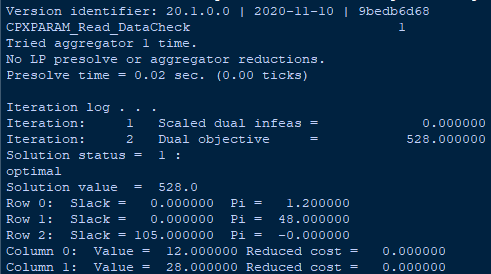
\includegraphics[width=10cm]{./images/Brasseur_Resolution.png}\label{Resultat_Brasseur}
 \caption{Résultat de l'optimisation du problème du brasseur}
 \end{center}
 \end{figure}

Nous voyons que nous avons pour revenu maximum 528 euro avec 12 unité de volume de bière blonde produite et 28 uinité de bière brune produites.

\subsection{Présentation de la résolution par backtracking}
L'algorithme du backtracking est plus précisément une famille d'algorithme qui sont utilisé le plus souent pour résoudre des problmèmes de satisfaction de contrainte.
Le backtracking est la solution la plus simple à comprendre il s'agit tout simplement de tester toutes les valeurs possible sur chaque case jusqu'a obtenir une sortie de sudoku remplie et valide.Cette algorithme agit comme un parcours d'arbre illustrons cela avec une image:\newline

\begin{figure}[h]
  \begin{center}
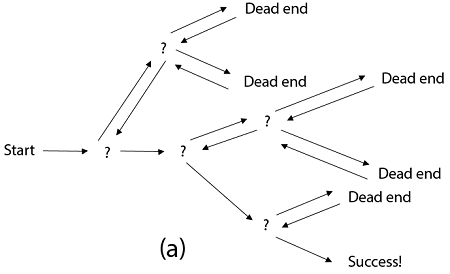
\includegraphics[width=10cm]{./images/backtracking.png}\label{Backtracking}
\caption{Illustration de l'algorithme du backtracking.}
\end{center}
\end{figure}

Comme l'illustre cette image nous essayons toutes les possibilitées et retournons en arrière si nous tombons dans une impasse dans nous passons de case vide\footnote{\label{vide}Une case vide est comme dit plus haut une case contenant la valeur 0} en case vide\footref{vide} en revenant en arrière si peu importe la le chiffre essayer dans cette case allant de 1 à 9, nous donne un sudoku invalide. Le problèlme de cette algorithme qui reviens le plus souvent est dù au fait que nous essayons toutes les valeurs possible ce qui nous donne une très grande quantité d'action et donc ce qui augmente considérablement notre temps de calcul nous pouvons toutefois régler ce problème en évitant de tester les possibiliter qui nous amène de façon logique à une impasse ou éviter de tester des possibilité d'une case si il est possible de déduire sa valeur de façonj logique.
\subsection{Pourquoi utiliser ces deux algorithme}

\subsubsection{Pourquoi utiliser l'algorithme du simplex}

La résolution avec l'algorithme du simplex permet une implementation intuitive et facililité dù à l'utilisation de Cplex. Cplex nous permet aussi une meilleur étude de la complexité de notre algorithme car cous pouvons voir les différentes itération de recherche de notre outil de résolution. Cette méthode de résolution nous permet aussi de revoir le problème de plusieur façon différente de par le fais que la résolution ne dépends que de nos contraintes.

\subsubsection{Pourquoi utiliser l'algorithme utilisant le backtracking}

La résolution avec avec backtracking est l'algorithme le plus naturel qui viennent à l'esprit dans la résolution de problème avec contrainte ce qui permet une facile implémentation de la gestion des contraintes malgré leur nombre.C'est un algorithme facilement améliorable car le but tout au long de son implémentation sera de tester le moins de valeur menant à une impasse possible. Cette algorithme a aussi pour avantage de n'avoir besoin daucune librairie extérieur ce qui permet une liberté totale au niveau du code et donne lieu à une certaine transparence quand à son fonctionnement contrairement aux fonctions que nous utilisons via cplex qui peuvent différé légèrement de leurs fonctionnements théoriques cités plus haut.

\subsection{Implémentation}
